\chapter[APÊNDICE \ref{Ap:CFD}]{Equações Governantes Da Mecânica Dos Fluidos}
\label{Ap:CFD}

%==================================================================================================
\section{Descrição Euleriana} \label{CFD-E}
%==================================================================================================

Em uma descrição Euleriana é possível se obter uma expressão que defina a conservação de massa (também denominada como Equação da Continuidade) do fluido, considerando um elemento infinitesimal permeável, que definirá o volume de controle, conforme ilustrado na Figura \ref{fig:BalMas}, em que $\mathbf{u}$ é o campo de velocidades e $\rho$ é a massa específica do fluido nesse ponto.

\begin{figure}[h!]
    \centering
    \caption{Taxa de fluxo de massa em um elemento infinitesimal permeável.}
    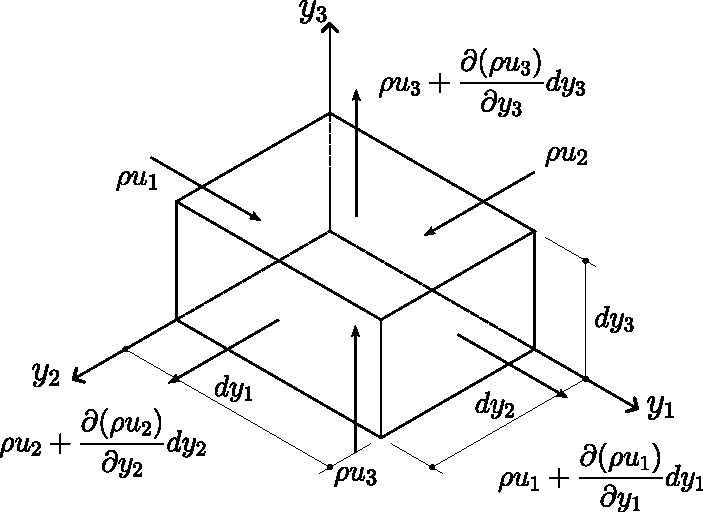
\includegraphics[width=.5\linewidth]{Figuras/BalMas.pdf}
    \\Fonte: Autoria Própria (\the\year).
    \label{fig:BalMas}
\end{figure}

Realizando-se o balanço de massa nesse elemento tem-se:

\begin{equation}
    dm=dm_0+\apder{dm}{t}dt\text{,}
\end{equation}

\noindent que, após algumas simplificações, resulta em uma expressão dada em sua forma simbólica de acordo com a Equação \ref{eq:BalMas1}, ou em notação indicial de acordo com a Equação \ref{eq:BalMas2}, que representam a conservação de massa em um elemento infinitesimal.

\textcolor{red}{Trocar $\bhat{e}_1$, $\bhat{e}_2$ e $\bhat{e}_3$ por $y_1$, $y_2$ e $y_3$. Não faz sentido adotar mais um sistema de coordenadas.}
\begin{subequations}
    \begin{equation}
        \frac{D\rho}{Dt}+\rho\NN\cdot\BB{u}=\apder{\rho}{t}+\NN\cdot(\rho\BB{u})=0\text{,}\label{eq:BalMas1}\\
    \end{equation}
    \begin{equation}
        \dot{\rho}+(\rho u_i)_{,i}=0\text{,}\label{eq:BalMas2}
    \end{equation}
    \label{eq:BalMas}
\end{subequations}

\textcolor{red}{Adote apenas uma notação para apresentar as equações nessa altura. Eu adotaria a simbólica e posteriormente, na hora de aplicar o mef, escreveria a forma indicial a ser usada, se julgar necessário. Aplique essa mesma lógica a todo o texto.}

\noindent sendo \noindent sendo que $\NN\cdot(\cdot)$ representa o divergente em relação às coordenadas atuais $\mathbf{y}$ e $D\rho/Dt$ é a derivada material, definida para um escalar $\phi$ qualquer como:

\begin{equation}
    \frac{D\phi}{Dt}=\apder{\phi}{t}+\BB{u}\cdot\NN\phi\text{,}
\end{equation}

\noindent onde $\NN(\cdot)$ representa o gradiente em relação às coordenadas atuais $\mathbf{y}$.

%
%, definido para uma função escalar $g$ qualquer de acordo com a Equação \ref{eq:grad1} e para uma função vetorial $\BB{g}$ qualquer de acordo com a Equação \ref{eq:grad2}:

%\begin{subequations}
%    \begin{equation}
%        \NN g=\der{g}{\BB{y}}\equiv\der{g}{y_i}=g_{,i}\text{,}\label{eq:grad1}
%    \end{equation}
%    \begin{equation}
%        \NN\BB{g}=\der{\BB{g}}{\BB{y}}\equiv\der{g_i}{y_j}=g_{i,j}\text{,}\label{eq:grad2}
%    \end{equation}
%\end{subequations}

%\noindent e $\NN\cdot(\cdot)$ é o divergente, que para uma função vetorial $\BB{g}$ qualquer, é dado por:

%\begin{equation}
%    \NN\BB{g}\equiv\der{g_i}{y_i}=g_{i,i}\text{,}
%\end{equation}

\noindent sendo a vírgula presente no subíndice a representação de derivada para a respectiva componente.

Para escoamentos incompressíveis a equação da continuidade pode ser reduzida a:

\begin{equation}
    u_{i,i}=0\text{,}\label{eq:incomp}
\end{equation}

\noindent denominada como condição de incompressibilidade.

Já a equação que expressa a Conservação da Quantidade de Movimento linear (ou de $Momentum$ Linear) pode ser obtida ao se considerar a taxa de fluxo de quantidade de movimento no elemento infinitesimal permeável, ilustrado na Figura \ref{fig:ConQtdMov}.

\begin{figure}[h!]
    \centering
    \caption{Taxa de fluxo de quantidade de movimento em um elemento infinitesimal permeável.}
    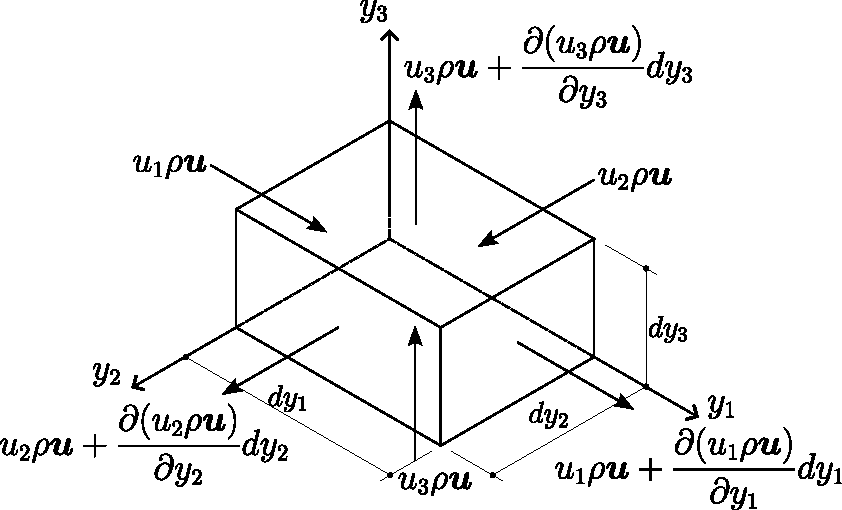
\includegraphics[width=.55\linewidth]{Figuras/ConQtdMov.pdf}
    \\Fonte: Autoria Própria (\the\year).
    \label{fig:ConQtdMov}
\end{figure}

Assim, procede-se com o balanço da taxa de quantidade de movimento, tendo-se uma resultante de forças externas atuante no elemento dado por $d\BB{F}$. Logo, após feitas as devidas simplificações, chega-se à equação:

\begin{equation}
    \apder{(\rho u_i)}{t}+(\rho u_ju_i)_{,j}-q_i=0\text{,}
    \label{eq:ConQtdMov}
\end{equation}

\noindent em que $q_i$ representa a força resultante por unidade de volume, ou seja, $q_i=dF_i/dV$. Entretanto, não é de interesse escrever a equação \ref{eq:ConQtdMov} em termos desse vetor $q_i$, mas em termos do tensor de tensões de Cauchy ($\sigma_{ij}$) e forças de volume. Para isso, considera-se o diagrama de corpo livre do elemento infinitesimal ilustrado na Figura \ref{fig:EqFor}, onde são representadas apenas as componentes de tensão e de forças de volume atuantes na direção $\bhat{e}_1$.

\begin{figure}[h!]
    \centering
    \caption{Componentes de forças atuantes no elemento infinitesimal na direção $\bhat{e}_1$.}
    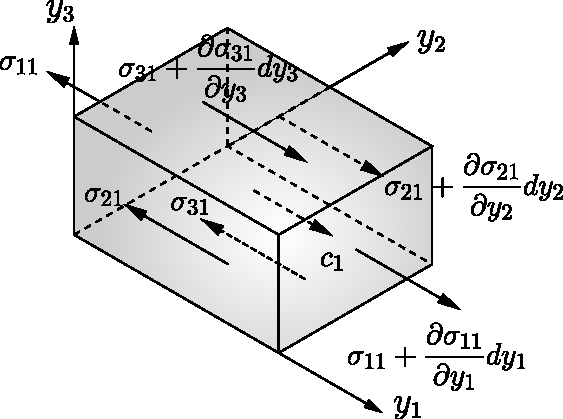
\includegraphics[width=.5\linewidth]{Figuras/EqFor.pdf}
    \\Fonte:Autoria Própria (\the\year).
    \label{fig:EqFor}
\end{figure}

Fazendo o equilíbrio de forças nessa direção, obtém-se que:

\begin{equation}
    q_1=\der{\sigma_{11}}{y_1}+\der{\sigma_{21}}{y_2}+\der{\sigma_{31}}{y_3}+c_1\text{,}
\end{equation}

\noindent a qual pode ser estendida analogamente para as demais direções como:

\begin{equation}
    q_i=\sigma_{ji,j}+c_i\text{.}
    \label{eq:RelQSig}
\end{equation}

Substituindo \ref{eq:RelQSig} em \ref{eq:ConQtdMov} e aplicando a condição de incompressibilidade obtém-se a equação da conservação da quantidade de movimento escrita em termos de tensões:

\begin{equation}
    \rho\bigpar{\dot{u}_i+u_ju_{i,j}-f_i}-\sigma_{ji,j}=0\text{,}
    \label{eq:ConQtdMov-2}
\end{equation}

\noindent em que $c_i=\rho f_i$, tal que $f_i$ é uma força por unidade de massa. Além disso, também é possível escrever a equação \ref{eq:ConQtdMov-2} utilizando a notação de derivada material como:

\begin{subequations}
    \begin{equation}
        \rho\bigpar{\frac{D\mathbf{u}}{Dt}-\mathbf{f}}-\NN\cdot\tens^T=\mathbf{0}\text{,}
    \end{equation}
    \begin{equation}
        \rho\bigpar{\frac{Du_i}{Dt}-f_i}-\sigma_{ji,j}=0\text{.}
    \end{equation}
    \label{eq:ConQtdMov-3}
\end{subequations}

Já o domínio em que essas equações são válidas pode ser definido como $\Omega\subset\mathbb{R}^{n_{sd}}$, sendo $n_{sd}=2$ ou $3$ a dimensão do problema em análise, tal que $\Omega$ possui uma fronteira $\Gamma=\partial\Omega$, em que a parte dessa fronteira onde se impõem condições cinemáticas é denominada como fronteira de Dirichlet ($\Gamma_D$) e a parte onde há prescrição de forças de superfície é denotado como fronteira de Neumann ($\Gamma_N$), conforme pode ser visualizado na Figura \ref{fig:Dom}.

\begin{figure}[h!]
    \centering
    \caption{Domínio de análise e fronteiras consideradas para problemas de mecânica dos fluidos.}
    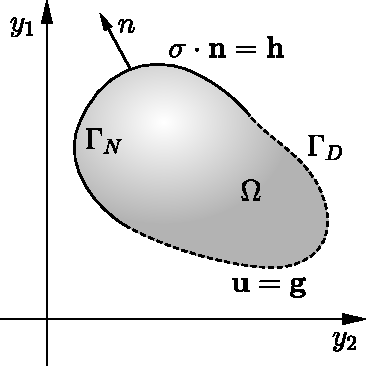
\includegraphics[width=.35\linewidth]{Figuras/Dom}
    \\Fonte: Autoria Própria (\the\year).
    \label{fig:Dom}
\end{figure}

Dessa forma, o problema a ser resolvido pode ser escrito a partir das equações:

\begin{equation}
    \left\{
    \begin{array}{ll}
        \rho\bigpar{\dot{u}_i+u_ju_{i,j}-f_i}-\sigma_{ji,j}=0 & \text{ em }\Omega\text{,}   \\
        u_{i,i}=0                                             & \text{ em }\Omega\text{,}   \\
        \sigma_{ij}n_i=h_j                                    & \text{ em }\Gamma_N\text{,} \\
        u_j=g_j                                               & \text{ em }\Gamma_D\text{,}
    \end{array}
    \right.\label{eq:NS-Euler}
\end{equation}

\noindent as quais são chamadas de equações de Navier-Stokes para escoamentos incompressíveis em descrição Euleriana \cite{bazilevs2013computational,bazilevs2010large,bazilevs2007variational,hughes2002variational,hughes2000large}.

%==================================================================================================
\section{Descrição Lagrangiana-Euleriana Arbitrária} \label{CFD-ALE}
%==================================================================================================

A descrição Lagrangiana-Euleriana Arbitrária (\textit{Arbitrary Lagrangian-Eulerian} - ALE) originou-se do trabalho de \citeonline{donea1982arbitrary}. São considerados 3 domínios, $\Omega_0$, $\Omega$ e $\hat{\Omega}$, que representam os domínios do contínuo em sua configuração inicial e atual e o domínio da malha respectivamente, como ilustrado na Figura \ref{Fig:ALE}. O domínio $\hat{\Omega}$ possui movimento arbitrário.

\begin{figure}[h!]
    \centering
    \caption{Descrição Lagrangiana-Euleriana Arbitrária.}
    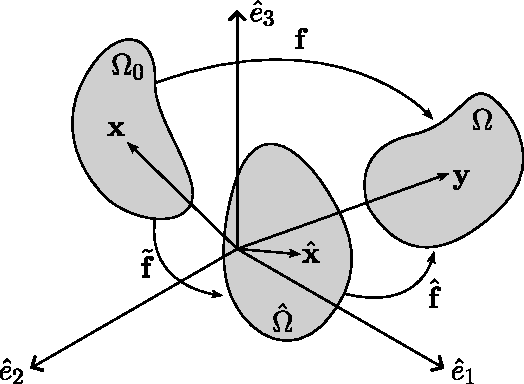
\includegraphics[width=.45\linewidth]{Figuras/ALE.pdf}
    \label{Fig:ALE}
    \\Fonte: Autoria Própria (\the\year).
\end{figure}

%\parei aquiiiii

As coordenadas $\BB{x}$, $\BB{y}$ e $\bhat{x}$ representam as coordenadas de um ponto nos domínios $\Omega_0$, $\Omega$ e $\hat{\Omega}$, respectivamente. Já as funções $\BB{f}(\BB{x},t)=\BB{y}(\BB{x},t)$, $\that{f}(\BB{x},t)=\bhat{x}(\BB{x},t)$ e $\bhat{f}(\bhat{x},t)=\BB{y}(\bhat{x},t)$ são funções de mudança de configuração.

Com isso, pode-se obter o gradiente das funções de mudança de configuração:

\begin{subequations}
    \begin{equation}
        \mathbf{A}=\der{(\BB{f}(\BB{x},t),t)}{(\mathbf{x},t)}=\begin{bmatrix}
            \der{\BB{y}}{\BB{x}} & \BB{u} \\\BB{0}^T&1
        \end{bmatrix}\text{,}\label{F2}
    \end{equation}
    \begin{equation}
        \that{A}=\der{(\that{f}(\BB{x},t),t)}{(\BB{x},t)}=\begin{bmatrix}
            \der{\bhat{x}}{\BB{x}} & \BB{w} \\\BB{0}^T&1
        \end{bmatrix}\text{, e}\label{F1}
    \end{equation}
    \begin{equation}
        \bhat{A}=\der{(\bhat{f}(\bhat{x},t),t)}{(\bhat{x},t)}=\begin{bmatrix}
            \der{\BB{y}}{\bhat{x}} & \uhat \\\BB{0}^T&1
        \end{bmatrix}\text{,}\label{F3}
    \end{equation}
    \label{eq:GradFun}
\end{subequations}

\noindent nos quais $\BB{u}=\partial\BB{y}/\partial t|_{\BB{x}}$, $\BB{w}=\partial\bhat{x}/\partial t|_{\BB{x}}$ e $\uhat=\partial\bhat{f}/\partial t|_{\bhat{x}}$. Além disso, vale ressaltar que $\BB{f}=\bhat{f}(\that{f},t)$, portanto $\BB{A}=\bhat{A}\cdot\that{A}$, ou seja:

\begin{equation}
    \begin{bmatrix}\der{\BB{y}}{\BB{x}}&\BB{u}\\\BB{0}^T&1\end{bmatrix}=
    \begin{bmatrix}\der{\BB{y}}{\bhat{x}}&\uhat\\\BB{0}^T&1\end{bmatrix}\cdot
    \begin{bmatrix}\der{\bhat{x}}{\BB{x}}&\BB{w}\\\BB{0}^T&1\end{bmatrix}\text{,}
    \label{F4}
\end{equation}

\noindent que possui, como uma de suas consequências:

\begin{equation}
    \BB{u}=\der{\BB{y}}{\bhat{x}}\cdot\BB{w}+\uhat\text{, ou}
    \label{u1}
\end{equation}

\begin{equation}
    \BB{w}=\der{\bhat{x}}{\BB{y}}\cdot(\BB{u}-\uhat)\text{.}
    \label{w1}
\end{equation}

Assim é possível definir a derivada material em uma descrição ALE. Para isso considere uma propriedade $\phi(\BB{y},t)$ escrita em termos da configuração atual, $\phi^*(\bhat{x},t)$ escrita em termos da configuração de referência e $\phi^{**}(\BB{x},t)=\phi^*(\that{f}(\BB{x},t),t)$ escrita em termos da configuração inicial. Logo:

\begin{equation}
    \der{\phi^{**}(\BB{x},t)}{(\BB{x},t)}=\der{\phi^*(\bhat{x},t)}{(\bhat{x},t)}\cdot\der{\that{f}(\BB{x},t)}{(\BB{x},t)}\text{, ou}
    \label{phi1}
\end{equation}

\begin{equation}
    \begin{bmatrix}\der{\phi^{**}}{\BB{x}}&\der{\phi^{**}}{t}\end{bmatrix}=
    \begin{bmatrix}\der{\phi^{*}}{\bhat{x}}&\der{\phi^{*}}{t}\end{bmatrix}\cdot
    \begin{bmatrix}\der{\bhat{x}}{\BB{x}}&\BB{w}\\\BB{0}^T&1\end{bmatrix}
    \text{.}
    \label{phi2}
\end{equation}

\noindent Portanto:

\begin{equation}
    \der{\phi^{**}}{t}=\der{\phi^{*}}{\bhat{x}}\cdot\BB{w}+\der{\phi^{*}}{t}\text{.}
    \label{phi3}
\end{equation}

Substituindo \ref{w1} em \ref{phi3}, obtém-se que:

\[\der{\phi^{**}}{t}=\der{\phi^{*}}{\bhat{x}}\cdot\der{\bhat{x}}{\BB{y}}\cdot(\BB{u}-\uhat)+\der{\phi^{*}}{t}\]

\[\der{\phi^{**}}{t}=\der{\phi^{*}}{t}+(\BB{u}-\uhat)\cdot\der{\phi^{*}}{\BB{y}}\]

Dessa maneira, remove-se os sobrescritos * e ** e define-se a derivada material na descrição ALE como:

\begin{equation}
    \frac{D\phi}{Dt}=\apderxh{\phi}{t}+(\BB{u}-\uhat)\cdot\NN\phi\text{.}\label{DerMat2}
\end{equation}

Com isso, substitui-se $\phi$ por $\rho$ e aplica-se a Equação \ref{DerMat2} em \ref{eq:BalMas} para se obter a Equação da Continuidade na descrição ALE:

\begin{equation}
    \apderxh{\rho}{t}+(\BB{u}-\uhat)\cdot\NN\rho+\rho\NN\cdot\BB{u}=0\text{,}
    \label{ConMas4}
\end{equation}

Já a Equação da Conservação da Quantidade de Movimento na descrição ALE pode ser obtida substituindo-se a Equação \ref{DerMat2} em \ref{eq:ConQtdMov-3}, em que $\mathbf{\phi}=\mathbf{u}$, obtendo-se:

\begin{equation}
    \rho\left(\apderxh{\BB{u}}{t}+(\BB{u}-\uhat)\cdot\NN\BB{u}-\BB{f}\right)-\NN\cdot\tens^T=\BB{0}\text{.}
    \label{ConQtdMov10}
\end{equation}

Assim, pode-se escrever o problema a ser resolvido a partir das equações:

\begin{equation}
    \left\{
    \begin{array}{ll}
        \rho\bigpar{\dot{u}_i+(u_j-\hat{u}_j)u_{i,j}-f_i}-\sigma_{ji,j}=0 & \text{ em }\Omega\text{,}   \\
        u_{i,i}=0                                                         & \text{ em }\Omega\text{,}   \\
        \sigma_{ij}n_i=h_j                                                & \text{ em }\Gamma_N\text{,} \\
        u_j=g_j                                                           & \text{ em }\Gamma_D\text{,}
    \end{array}
    \right.\label{eq:NS-ALE}
\end{equation}

\noindent que são denominadas como as equações de Navier-Stokes para escoamentos incompressíveis em descrição ALE \cite{bazilevs2013computational}.

%==================================================================================================
\section{Modelo Constitutivo} \label{MC}
%==================================================================================================

O modelo constitutivo que relaciona o tensor de tensões de Cauchy com os campos de velocidade e de pressão é expresso de acordo com a Equação \ref{eq:const1}:

\begin{equation}
    \sigma_{ij}=\tau_{ij}-p\delta_{ij}\text{,}\label{eq:const1}
\end{equation}

\noindent no qual $\tau_{ij}$ é o tensor de tensões viscosas (ou tensor desviador), que para fluidos Newtonianos é dado por:

\begin{equation}
    \tau_{ij}=\script{D}_{ij\alpha\beta}\dot{\varepsilon}_{ij}\text{,}
\end{equation}

\noindent em que $\script{D}_{ij\alpha\beta}$ é o tensor constitutivo de quarta ordem:

\begin{equation}
    \script{D}_{ij\alpha\beta}=2\mu\delta_{i\alpha}\delta_{j\beta}+\lambda\delta_{ij}\delta_{\alpha\beta}\text{,}
\end{equation}

\noindent sendo $\mu$ a viscosidade dinâmica do fluido e $\dot{\varepsilon}_{ij}$ é o tensor de taxa de deformação, definido como:

\begin{equation}
    \dot{\varepsilon}_{ij}=\frac{u_{i,j}+u_{j,i}}{2}\text{.}\label{eq:deftax1}
\end{equation}

Assim, o tensor desviador pode ser escrito da seguinte maneira:

\[\tau_{ij}=(2\mu\delta_{i\alpha}\delta_{j\beta}+\lambda\delta_{ij}\delta_{\alpha\beta})\dot{\varepsilon}_{\alpha\beta}=2\mu\delta_{i\alpha}\delta_{j\beta}\dot{\varepsilon}_{\alpha\beta}+\lambda\delta_{ij}\delta_{\alpha\beta}\dot{\varepsilon}_{\alpha\beta}\]

\noindent resultando em:

\begin{equation}
    \tau_{ij}=2\mu\dot{\varepsilon}_{ij}+\lambda\dot{\varepsilon}_{\beta\beta}\delta_{ij}\text{.}
\end{equation}

Já para o caso de escoamentos incompressíveis, verifica-se que $\dot{\varepsilon}_{\beta\beta}=0$, fazendo com que \ref{eq:const1} possa ser escrita como:

\begin{equation}
    \sigma_{ij}=\mu(u_{i,j}+u_{j,i})-p\delta_{ij}\text{.}\label{eq:ModConst}
\end{equation}